\chapter{Electronics Design}
\label{ch:electronics}
%Electronics section overview ...

\begin{figure}[H]
	\begin{center}
		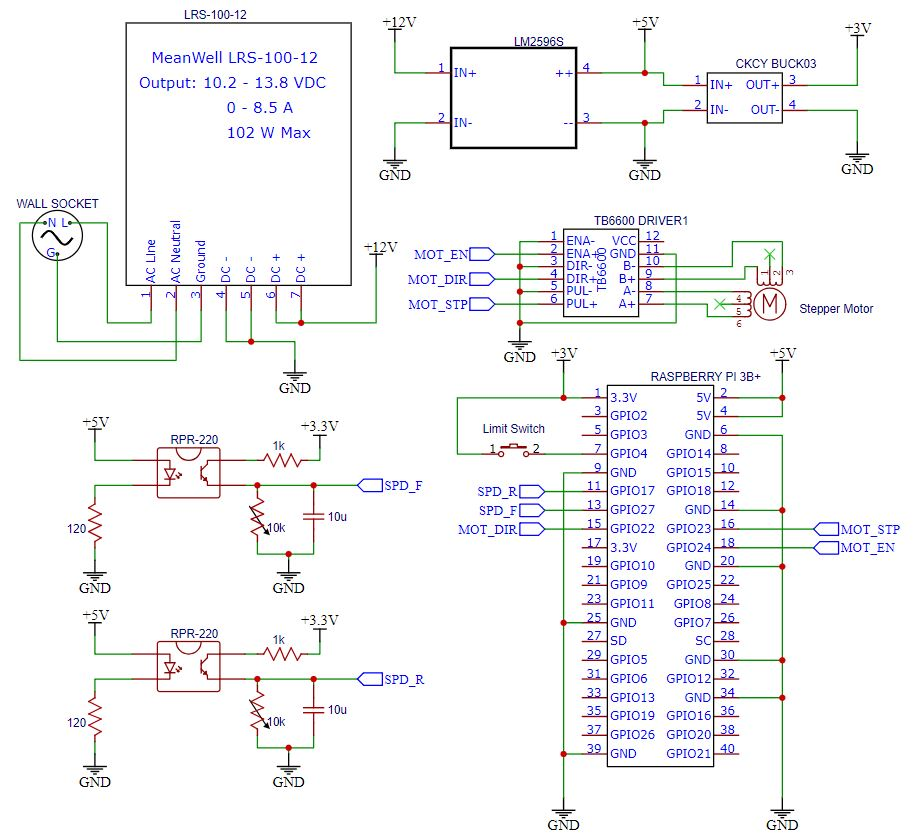
\includegraphics[width=0.9\textwidth]{Circuit.jpg}
		\caption{Electronics Circuit Diagram}
		\label{fig:circ}
	\end{center}
\end{figure}

\section{Speed Sensor Design}

Optical rotary encoder tachometers are used to measure the speed of the rollers on the rear section of the frame. Figure~\ref{fig:rpr} shows the RPR-220 infrared photo-transceiver units that were used. These units consist of an infrared lamp and a phototransistor in a plastic housing. The configuration can be seen in Figure~\ref{fig:sensorD}.

\begin{figure}[H]
	\centering
	\begin{subfigure}[t]{.35\textwidth}
		\centering
		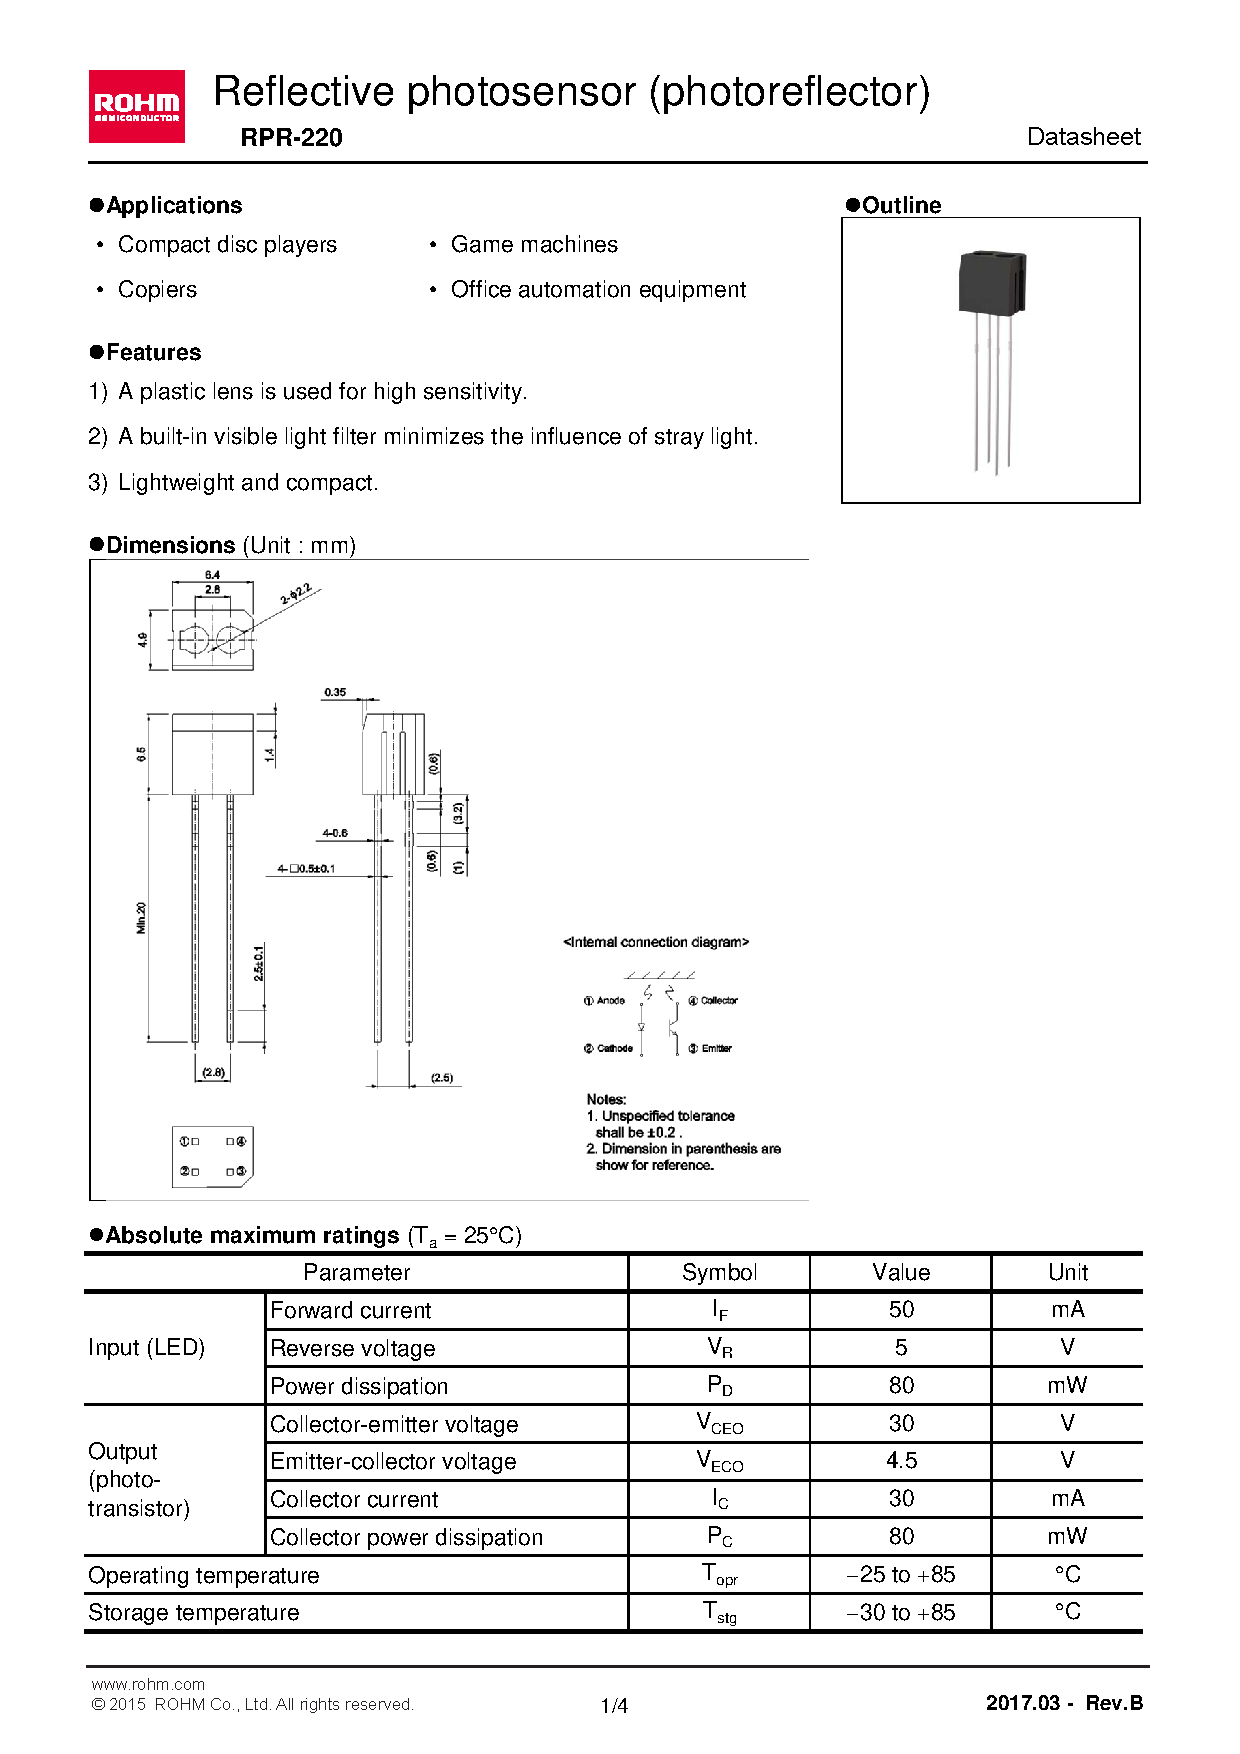
\includegraphics[width = 0.8\linewidth]{RPR220.jpg}
		\caption{RPR-220 Photo-Transceiver}
		\citep[2015]{RPR:2015}
		\label{fig:rpr}
	\end{subfigure}
\hfill
	\begin{subfigure}[t]{.6\textwidth}
		\centering
		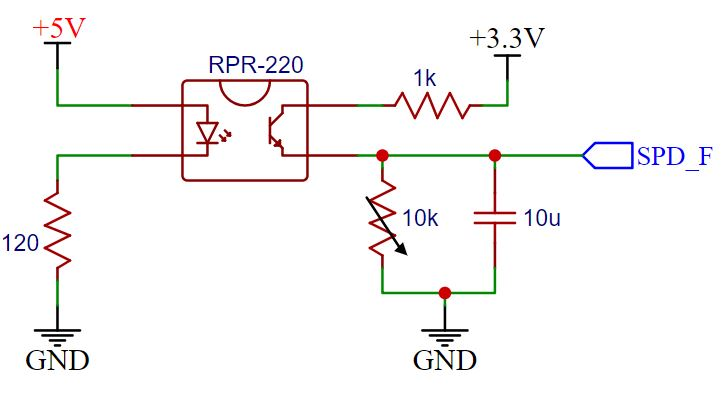
\includegraphics[width = 0.8\linewidth]{SensorCircuit.JPG}
		\caption{Sensor Biasing and Filter Circuit}
		\label{fig:sensorD}
	\end{subfigure}
	\caption{Sensor Design}
	\label{fig:Sensor}
\end{figure}

\vspace*{-1cm}

\subsection{Transistor Biasing}

The phototransistor has a rated collector current ($I_c$) of \SI{0.3}{\milli\ampere} if \SI{90}{\percent} reflection is achieved at a distance of \SI{6}{\milli\meter}. A voltage divider circuit was used to achieve a \SI{3.3}{\volt} reading on the output to the Raspberry Pi \ac{gpio} pin allowing for the signals to be read as a digital input. This eliminates the need for an analog to digital conversion channel. Equation~\ref{eq:ohm} is used to determine the required resistance.

\begin{equation}
	R = \frac{V}{I}
	\label{eq:ohm}
\end{equation}

Using Equation~\ref{eq:ohm}, a resistance ($R$) of \SI{11}{\kilo\ohm} was determined. Figure~\ref{fig:sensorD} shows how a \SI{10}{\kilo\ohm} variable resistance potentiometer was placed in series with a \SI{1}{\kilo\ohm} resistor, allowing for tuning of the biasing circuit based on individual transistor fluctuations or operating conditions. 

In order to produce more reliable readings, a first-order low-pass RC filter was implemented. Designing for a cut-off frequency ($f_c$) of \SI{10}{\kilo\hertz}, Equation~\ref{eq:freq} is used to determine the required capacitance value ($C$) of \SI{10}{\micro\farad}.

\begin{equation}
	f_c = \frac{1}{2 R C}
	\label{eq:freq}
\end{equation}

\subsection{Encoder Design}

The ``Rpi.GPIO'' library on the Raspberry Pi allows for interrupt activated measurements up to \SI{5}{\kilo\hertz}. The maximum expected speed of the rollers is determined to be 3000 \ac{rpm} or \SI{50}{\hertz}. Since a digital input is used to measure the rotations, there will be some bounce cases where a single input might be measured more than once. 

In order to eliminate this, software de-bouncing is implemented with a delay of \SI{1}{\milli\second}. This means that the readable frequency is reduced to \SI{1}{\kilo\hertz}. An encoder disk with 10 segments would allow for a safety factor of 2. Figure~\ref{fig:spdDisk} shows the encoder disk that was used to create the tachometers.

\begin{figure}[H]
	\centering
	\begin{subfigure}[t]{.3\textwidth}
		\centering
		
\includegraphics[width = \linewidth]{MeasureWheel.jpg}
		\caption{Rotary Encoder Disk}
		\label{fig:spdDisk}
	\end{subfigure}
\hfill
	\begin{subfigure}[t]{.65\textwidth}
		\centering
		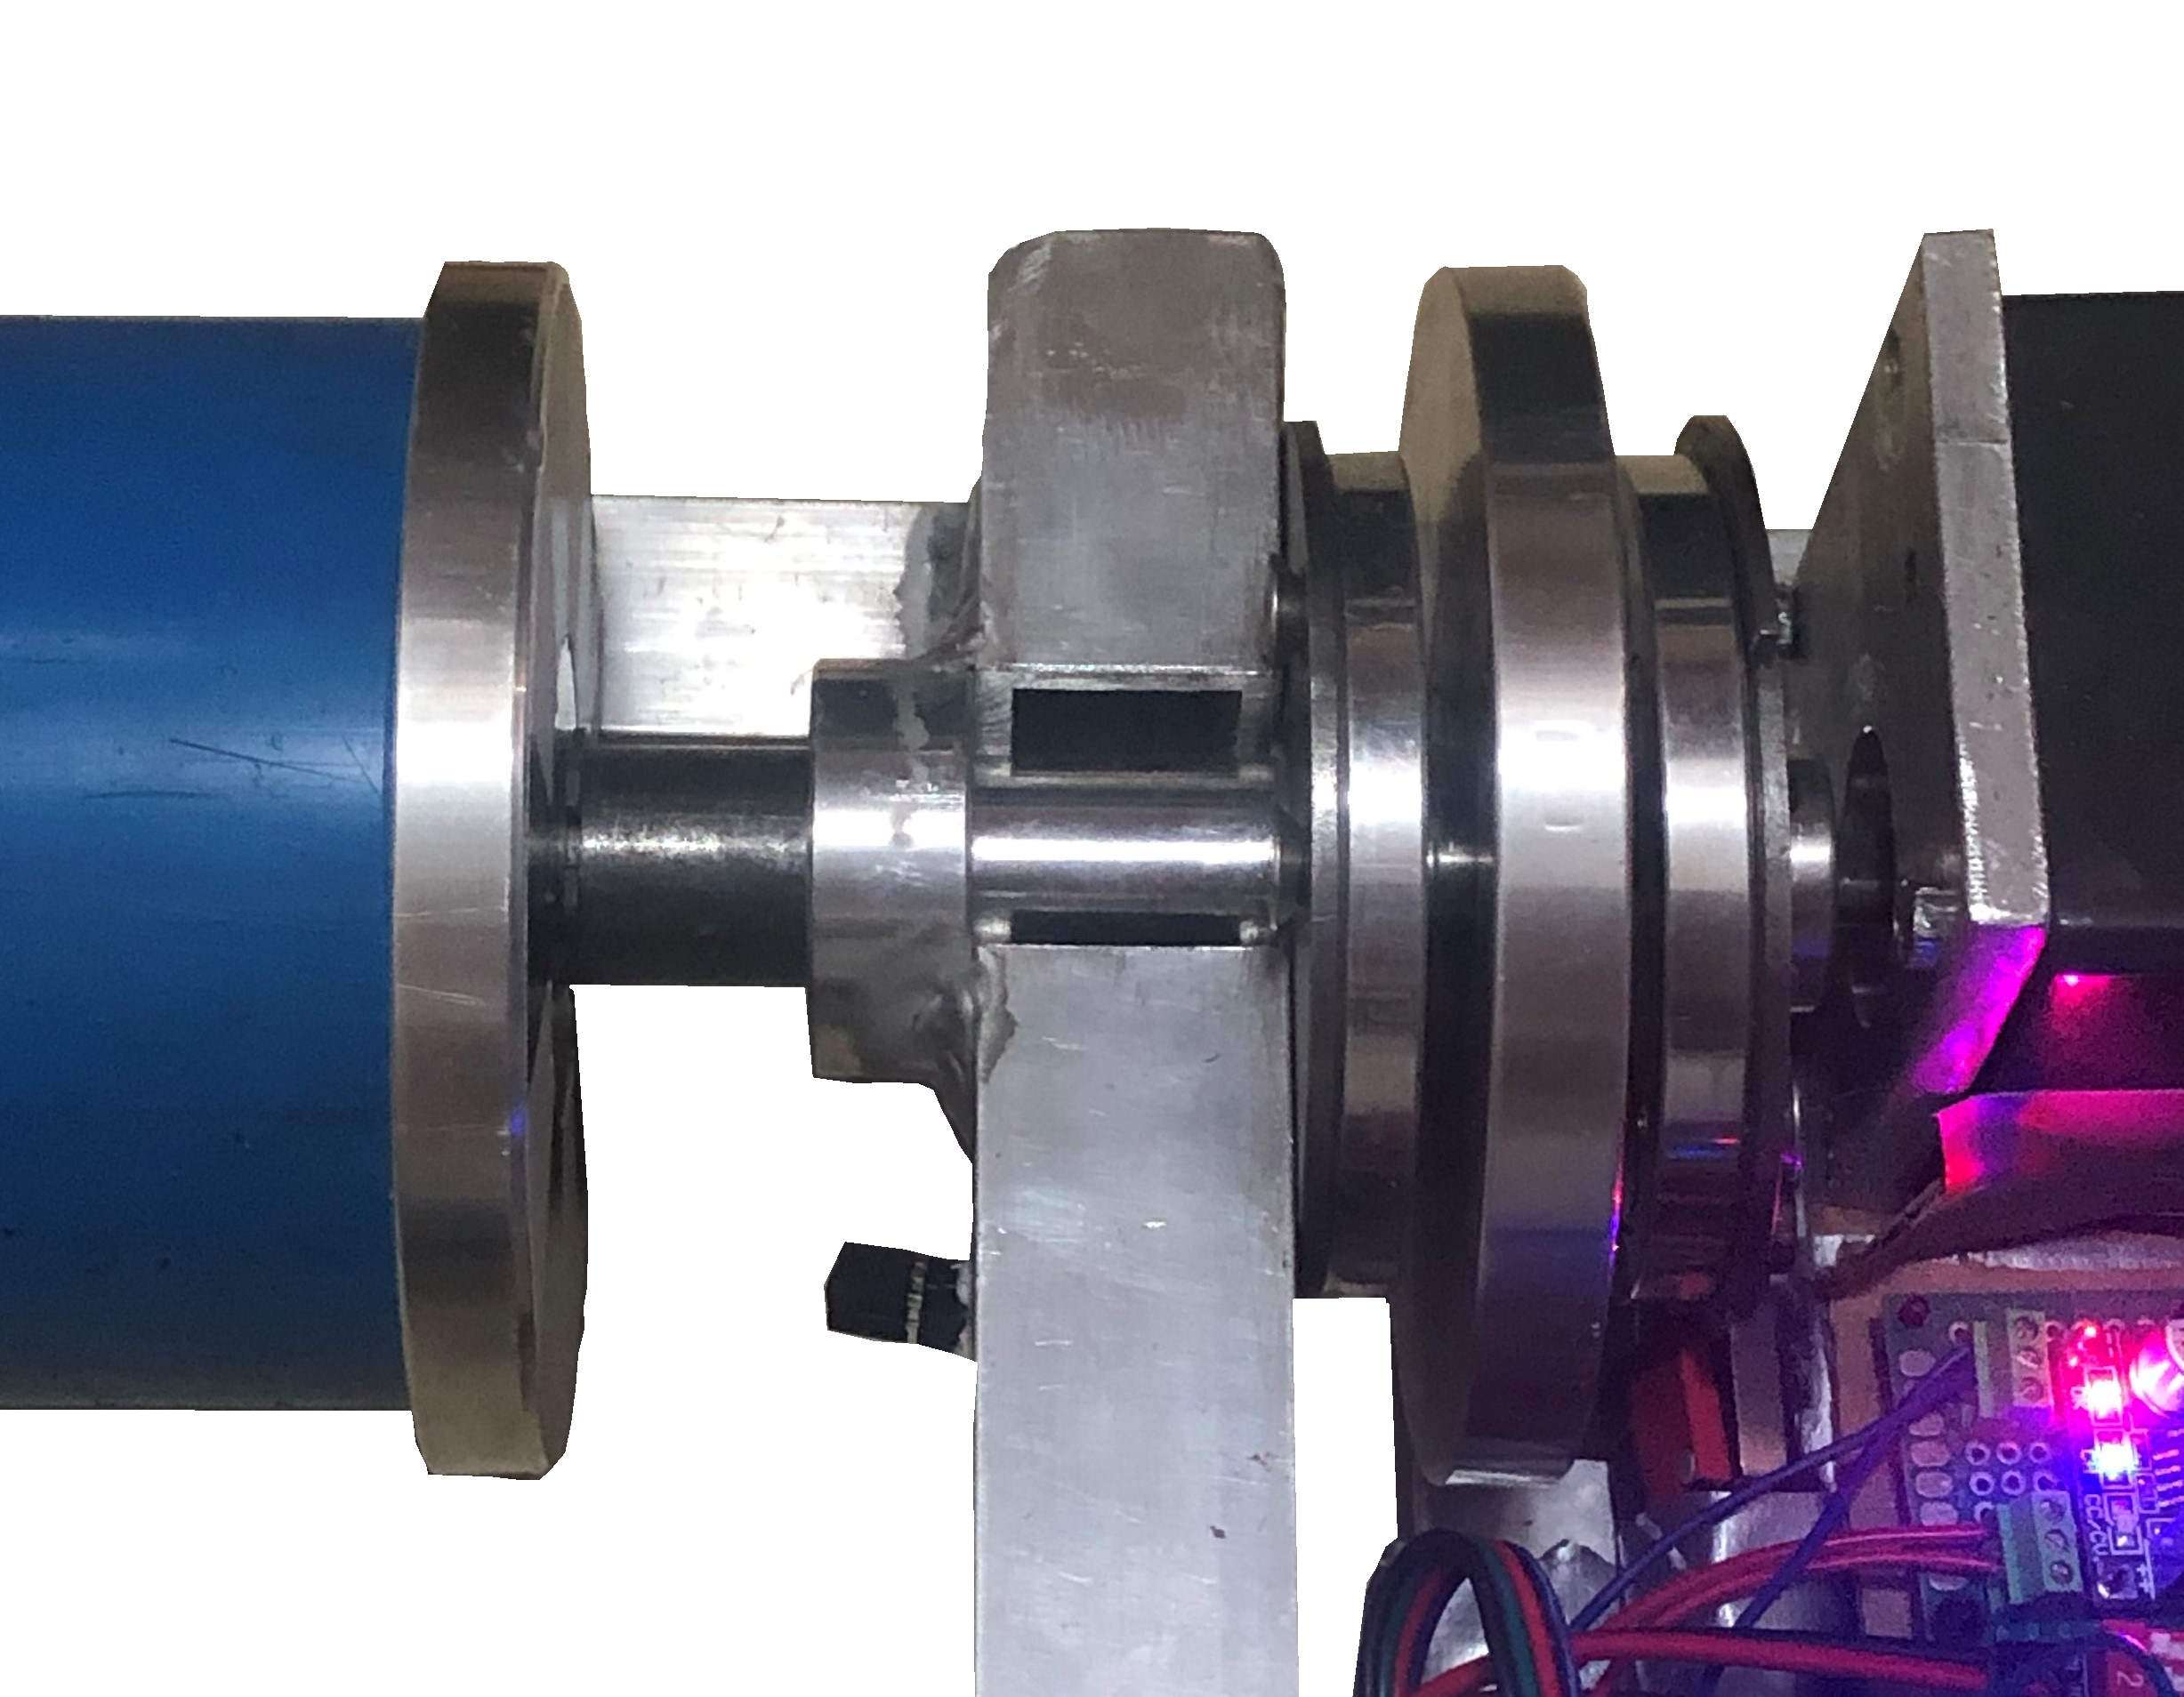
\includegraphics[width = 0.9\linewidth]{speedSensor.jpg}
		\caption{Constructed Speed Sensor}
		\label{fig:spdSensor}
	\end{subfigure}
	\caption{Speed Sensor}
	\label{fig:spd}
\end{figure}

\vspace*{-0.5cm}

Figure~\ref{fig:spdSensor} shows the final constructed tachometer with the wires routed inside of the trainer frame.

\section{Motor Control}

In order to change the phase alignment of the magnet arrays of the eddy current brake, one magnet array is mounted to a stepper motor. In order to handle the torque requirements and provide a larger degree of control for the brake, a Nema-23 motor with a 15:1 reduction gearbox was used. The motor and gearbox, shown in Figure~\ref{fig:stepper}, is driven by a TB660 stepper motor driver shown in Figure\ref{fig:motorDriver}.

\begin{figure}[H]
	\centering
	\begin{subfigure}[t]{.550\textwidth}
		\centering
		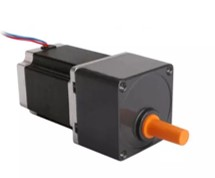
\includegraphics[height = 3cm]{StepperMotor.jpg}
		\caption{Nema 23 Stepper Motor with 15:1 Gearbox}
		\citep{Robotics:2022}
		\label{fig:stepper}
	\end{subfigure}
	\begin{subfigure}[t]{.41\textwidth}
		\centering
		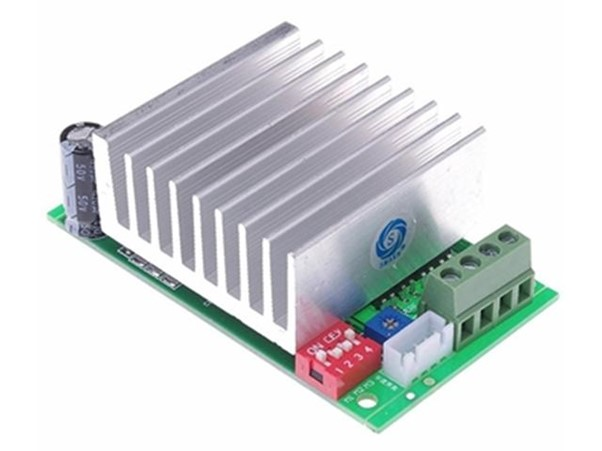
\includegraphics[height = 2.5cm]{StepperDriver.jpg}
		\caption{TB660 v1.1 Stepper Motor Driver}
		\citep{Communica:2022}
		\label{fig:motorDriver}
	\end{subfigure}
	\caption{Motor Components}
	\label{fig:Motor}
\end{figure}

\vspace*{-0.5cm}

\section{Electronics Overview}

Figure~\ref{fig:circ} is the circuit diagram that was designed and implemented for the trainer. A LRS \SI{100}{\watt}, \SI{12}{\volt} power supply is used to supply the entire circuit with DC power. The \SI{12}{\volt} supply is then stepped down to \SI{5.5}{\volt} and \SI{3}{\volt} by LM2596S and CKCY Buck03 voltage regulators respectively before being distributed to the remaining circuit.

Figure~\ref{fig:elecAll} shows the final construction of the electronics of the trainer. The components are mounted on cardboard cut-outs that serve as insulation between the aluminium frame and the components. 

\begin{figure}[H]
	\centering
	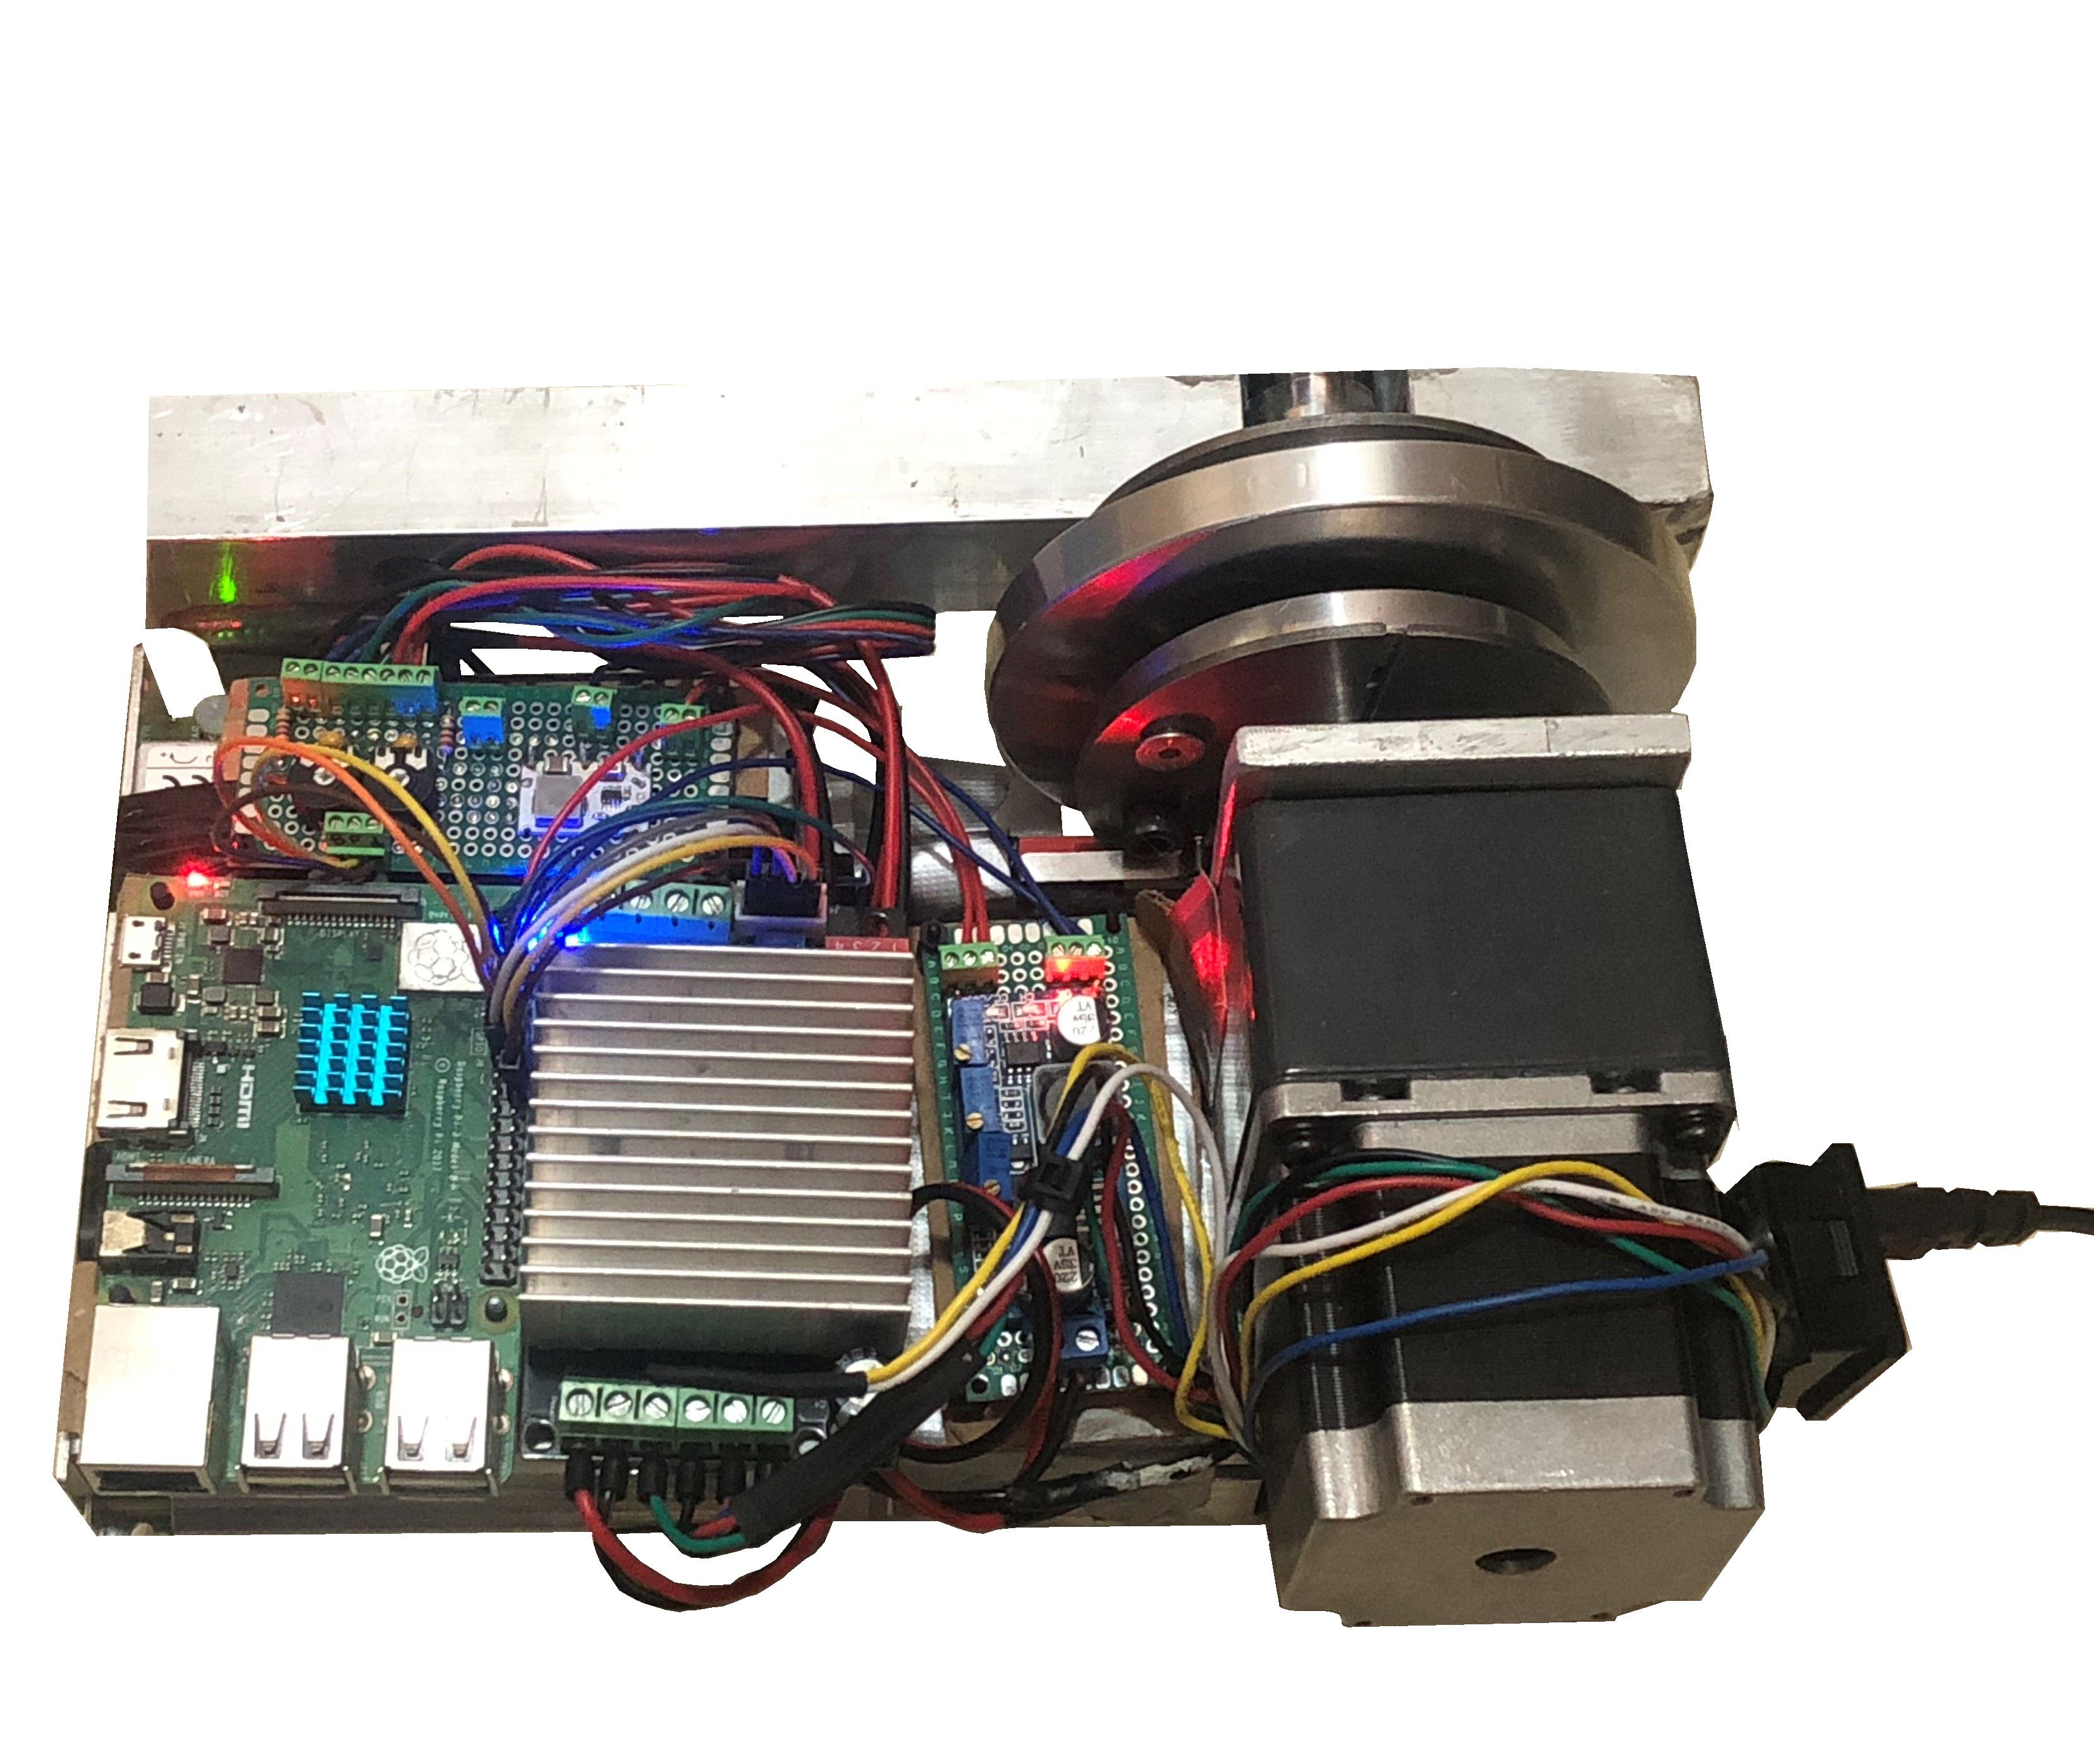
\includegraphics[width=0.8\textwidth]{electronics.jpg}
	\caption{Electronics Construction}
	\label{fig:elecAll}
\end{figure}

Since the developed model serves as a proof of concept, components were not permanently mounted. This allows for rapid testing and replacing of components.
